Thus far, we have outlined our approaches to fiducial detection in the previous sections.
In this sections, we evaluate our algorithms on three state of the art datasets
LFPW, COFW and AFLW. Before we present the quantitative result (produced in Table~\ref{table:ourBestResults_mean}) in the remaining
part of this section, we describe the 3 datasets in brief below. 
 
% \begin{figure}
%   \centering
%   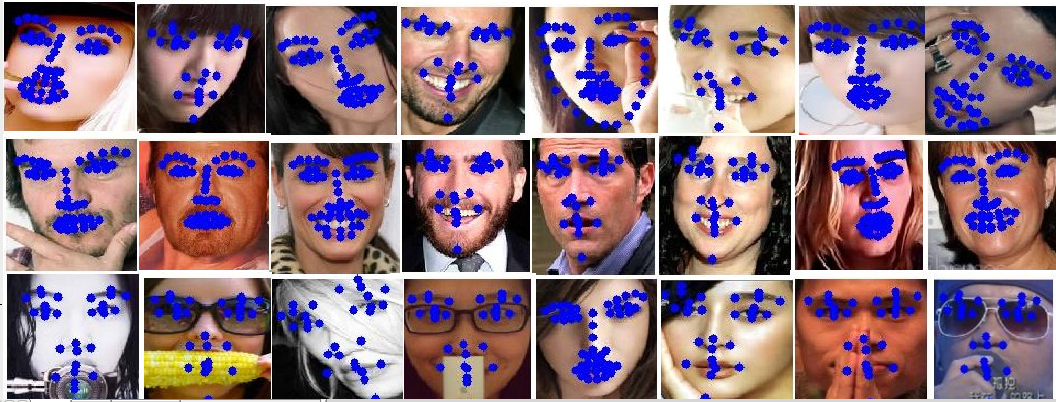
\includegraphics[width=3in,height=1.2in]{figures/pose_expression_occlusion.png}
%   \caption{Results with varying pose (Row 1), expression (Row 2) and 
%   occlusion (Row 3). Best viewed in color.}
%   \label{fig:sample_results}
% \end{figure}
 

We have chosen 3 popular datasets to test the performance of our algorithm for several reasons.

\subsection{LFPW}
is the oldest dataset we consider~\cite{kumarPAMI13_faceExem}, and contains faces of several people in ``wild'' settings,
with lots of occlusions and pose / expression variation. It contains 1035 images, out of which
811 are used for training and 224 are used for testing purposes. Ground truth annotation of
training images in the form of 68 fiducial locations for each face is available to us. This dataset
has been standard for some time, but current algorithms give very good performance 
on it.

\subsection{COFW}
is a dataset released by Burgos-Artizzu \etal~\cite{artizzzuICCV13_COFW}, and is
specialzed to highlight situations where faces are occluded in a manner
that hinders accurate fiducial detection by state-of-the-art algorithms.
It contains 1852 images, out of which
1345 are used for training and 507 are used for testing purposes. Ground truth annotation of
training images in the form of 29 fiducial locations for each face is available to us. This dataset
is relatively new, and moderate performances have been reported on it.

\subsection{AFLW}
is a dataset released by~\cite{koetsingerBFIAT11_AFLW}, and contains several annotated face images
in extreme settings. It is considered one of the toughest datasets in fiducial detection
literature~\cite{smithECCV14_ED,zhangECCV14_deepfacealign}, as it has larger pose variations, 
partial occlusions and illumination variation compared to other datasets. Like
~\cite{zhangECCV14_deepfacealign}, we sample 1000 training images and 3000 testing images
randomly from the dataset, while ensuring no overlap between the two sets.

